\subsection{階層型NNによる学習}
\subsubsection{最適なパラメータを探すためのアプローチ}
% 指定された条件下において学習が効率良く行われるパラメータの組み合わせを探
% すため、**して**することでパラメータを調整した。
% 
% (補足:全パターンを調べても良いし、いくつかのパターンを調べても良いが、
% どのような方法で調整したら良いかを考えよう)

$ETA,ALPHA,HIDDEN$を指定された範囲内でランダムな値に設定し,
プログラムを実行した.
パラメータの値の決定や,iteration数の平均値を求める処理は
次のシェルスクリプト(ソースコード\ref{level2})で行った.
ExOR問題は線形分離不可であるため,HIDDENの最小値を2としている.
最大値は特に指定されていないが,HIDDENを極端に大きくしすぎると
各パラメータの最適な組み合わせを見つけ出すのが困難になると考えたため,
最大値を16とした.


\lstinputlisting[caption=本levelで使用したシェルスクリプト,label=level2]{./level2figs/level2.sh}

このシェルスクリプトを数十回実行し,
iteration数の平均値が比較的小さい実行結果を10個分記録した.
その中で平均値が最小なものを選択し,グラフ化することにした.
%また出力結果の文字列を処理するため,
%bp\_mo\_exor.cの終了条件$FINISH$を出力するfprintf関数のstderrをstdoutへと変更を行った(ソースコード\ref{exor}).
%
%\lstinputlisting[caption=bp\_mo\_exor.cの変更点,label=exor]{./level2figs/exor.c}
%

\subsubsection{実行結果}

% (補足:シード値10パターンで試した際の収束に要した学習回数と、その平均回数が分かるように明示してください。)

表\ref{table:level2}にシード値10パターンで試した際の収束に要した学習回数と,その最小の平均回数を示す.

\begin{table}[htb]
 \begin{center}
  \begin{tabular}[htb]{|r|l|} \hline
   シード値 & 収束した回数 \\ \hline \hline
   1000     & 37\\ \hline
   2000     & 45\\ \hline
   3000     & 52\\ \hline
   4000     & 44\\ \hline
   5000     & 50\\ \hline
   6000     & 53\\ \hline
   7000     & 39\\ \hline
   8000     & 29\\ \hline
   9000     & 38\\ \hline
   10000    & 39 \\ \hline \hline
   10試行の平均値 & 42 \\ \hline
  \end{tabular}
  \caption{階層型NNによるExOR問題の学習に要した回数}
  \label{table:level2}
 \end{center}
\end{table}

各パラメータが$ETA=1.26, ALPHA=0.94, HIDDEN=16$の時,表\ref{table:level2}のような結果が得られた.
その時の学習曲線は図\ref{fig:averageultimate}のようになる.
図\ref{fig:averageultimate}はgnuplotを用いてseed値別にプロットしたグラフを元にsmooth uniqueオプションで平均化を行い,得られたものである.

\begin{figure}[h]
 \begin{center}
  \includegraphics[width=10.0cm]{./level2figs/averageultimate.eps}
  \caption{重みを更新する様子(平均値)}
  \label{fig:averageultimate}
 \end{center}
\end{figure}


\subsubsection{考察}
ここでは,各パラメータとiteration数の関係について考察する. \\
 下記に平均iteration数が比較的小さい実行結果とそのときのパラメータの値を示す.
\begin{itembox}[c]{平均iteration数が小さい実行結果}
    {\small
        \verbatimtabinput{./level2figs/suitables.txt}
    }
\end{itembox}
10回の実行結果における共通点は,いずれもALPHA値が1に近い値をとるという点だった. \\
 続いて,平均iteration数が大きい実行結果を示す.

\begin{itembox}[c]{平均iteration数が大きい実行結果}
    {\small
        \verbatimtabinput{./level2figs/unsuitables.txt}
    }
\end{itembox}

平均iteration数が小さいときのパラメータと平均iteration数が大きいときのそれとを比較すると,
HIDDENの値が小さいと平均iteration数が大きくなり,
反対に値が大きいと平均試行回数が小さくなるという結果になった.
また$ETA$に関しては,0を設定しない限りiteration数に大きな影響を
与えないことが伺える.
%また,$ETA$の値が0だと学習回数が100000を越える結果となった.
%これら実行結果より,$ETA,ALPHA,HIDDEN$は
これら実行結果より,最も効率良く学習が収束するパラメータの組み合わせは,表\ref{table:parameters}のようになる.

\begin{table}[htb]
 \begin{center}
  \begin{tabular}[htb]{|c|c|c|} \hline
   $ETA$ & $ALPHA$ & $HIDDEN$ \\ \hline \hline
   0以外の数値 & 1に近い値 & できるだけ大きい数値\\ \hline
  \end{tabular}
  \caption{最適なパラメータの組み合わせ}
  \label{table:parameters}
 \end{center}
\end{table}
